\documentclass[letterpaper,10pt,serif,draftclsnofoot,onecolumn,compsoc,titlepage]{IEEEtran}

\usepackage{graphicx}                                        
\usepackage{amssymb}                                         
\usepackage{amsmath}                                         
\usepackage{amsthm}                                          
\usepackage{cite}
\usepackage{alltt}                                           
\usepackage{float}
\usepackage{color}
\usepackage[hyphens]{url}
\usepackage{pgfgantt}
\usepackage{rotating}
\usepackage{enumitem}
\usepackage{gensymb}
\usepackage[T1]{fontenc}

\usepackage{balance}
\usepackage[TABBOTCAP, tight]{subfigure}
\usepackage{enumitem}

\usepackage{geometry}
\geometry{margin=.75in}
\usepackage{hyperref}
\usepackage{breakurl}
%\usetikzlibrary{shapes, positioning, calc}
\usepackage{caption}
\usepackage{listings}
%\usepackage[utf8]{inputenc}
%pull in the necessary preamble matter for pygments output

\usepackage{listings}
\definecolor{dkgreen}{rgb}{0,0.6,0}
\definecolor{gray}{rgb}{0.5,0.5,0.5}
\definecolor{mauve}{rgb}{0.58,0,0.82}

\lstset{frame=tb,
  %language=Java,
  aboveskip=3mm,
  belowskip=3mm,
  showstringspaces=false,
  columns=flexible,
  basicstyle={\small\ttfamily},
  numbers=none,
  %numberstyle=\tiny\color{gray},
  %keywordstyle=\color{blue},
  %commentstyle=\color{dkgreen},
  %stringstyle=\color{mauve},
  breaklines=true,
  breakatwhitespace=true,
  tabsize=3
}

%% The following metadata will show up in the PDF properties
\hypersetup{
   colorlinks = true,
   citecolor = black,
   linkcolor = black,
   urlcolor = black,
   breaklinks = true,
   pdfauthor = {Shu-Ping Chien, Brock Smedley, W Keith Striby Jr},
   pdfkeywords = {CS461 "Senior Project" Progress Report},
   pdftitle = {CS461 Winter Midterm Progress Report},
   pdfsubject = {CS461 Winter Midterm Progress Report},
   pdfpagemode = UseNone
}

\parindent = 0.0 in
\parskip = 0.1 in
\title{Winter Midterm Progress Report: Multi-Camera, SoM Based, Real-Time Video Processing for UAS and VR/AR Applications}
\author{Area 51: Shu-Ping Chien, Brock Smedley, W Keith Striby Jr \\ 16 February 2018 \\ CS461, Senior Software Engineering Project, Winter 2018}


\begin{document}
\begin{titlepage}
\maketitle

\begin{abstract}

This document highlights the group's progress made during the first half of the 
Winter 2018 term. The project is introduced along with an explanation of the 
hardware and software surrounding our product's planned solution. Then each group member
explains their contributions to the project, what they have remaining to complete
the projects requirements, and problems experienced with solutions if applicable. \\


\thispagestyle{empty}
\end{abstract}
\end{titlepage}

\newpage
\tableofcontents

\newpage

\section{Introduction}

\subsection{Purpose}
Our project is required to provide a video output at near real-time from a 
multi-camera input utilizing an NVIDIA Jetson TX1 or TX2 system-on-module (SoM). 
The software produced will perform image processing and edge computing on the 
camera input to display a visually enhanced and stitched video output. 
Size, weight, power, and cost (SWaP-C) requirements for the project are due 
to its application being for UAS and VR/AR, and from our system utilizing a 
mass-produced SoM, particularly the Jetson TX1 or TX2. \\

\subsection{Scope}
Application specific hardware and software are vital for the project due the the 
system requirements and constraints of the project.
The NVIDIA Jetson TX1 and TX2 run on an Ubuntu based Linux for Tegra (L4T) operating 
system created specifically for producing customized imaging, installed on a 
GPU-accelerated dual-core CPU with dual Image Signal Processors (ISPs). \\

L4T, being an Ubuntu variant, provides a friendly development interface with access to a 
large repository of additional software.
NVIDIA provides the Jetson Software Development Pack (JetPack) 3.1 which has L4T 28.1 
and is capable of supporting a multitude of multimedia and image processing API. Jetpack 
is installed on an Ubuntu host computer and is then used to flash the TX2's memory with L4T and 
selected libraries. \\

The cameras will utilize the most widely used camera interface for mobile applications, 
MIPI CSI-2, which is capable of supporting 1080p, 4k, and 8k video. 
A carrier board will connect the cameras to the Jetson TX1 or TX2 that also provides 
additional application-specific interfaces and peripherals. \\

The software materials for this project will support the NVIDIA Jetson TX1 and TX2 and 
be able to produce fused images from cameras in near real-time. The media inputs from 
cameras through CSI will be captured in pipelines for distribution and transformation 
then sent to the image processor, and the process avoids to reload our input datas to 
reduce latency. The image processing software will utilize the images from media stream 
and produce stitched images as output to the display device.  \\

\subsection{Overview}
This document provides a recap of the progress made on our project through the first half
of the Winter 2018 term. The group so far has been primarily focused on getting the TX2 module to produce a multi-camera output with a CSI (Camera Serial Interface) module attached to the TX2 module, which allows us to connect multiple cameras to the device.
Shu-Ping Chien and W Keith Striby Jr have primarily been working in tandem so their 
contributions will be similar. Brock has spent most of the term doing research about the software we use so that it may later be scripted in order to save development time. The following 
sections reflect this progress with each group member explaining where their involvement 
with the project currently is, work remaining, and problems experienced so far over the term 
with solutions if applicable. \\ 


\section{Contributor: Shu-Ping Chien}

\subsection{Current Project Status}

In the first five weeks, the group try to capture images from Raspberry Pi v2.1 cameras 
through the CSI-2 camera ports, and the group recorded each attempt and process in document. 
At the end of week five, the group has explored on different methods to activate the cameras 
through J20 CSI-2 board, but the result was not as ideal as expected to solve the majority 
problem of images capturing. In each re-flashing attempt, the group added patches for Auvidea 
J106 board and re-flash Jetpack to TX2 module, then build up kernel to see if the connection 
with cameras and pipeline worked.\\

In the last progression, the group was able to set up patches for Auvidea J106 carrier board 
and the Auvidea M110 motherboard in order to connects the board together with the monitor and 
enable keyboard and mouse. It was successful after building the kernel on TX2 module, but the 
applied patches for IMX-219 driver, which is a driver released by RidgeRun to activate Raspberry 
Pi camera through J20 CSI-2 board for NVIDIA TX1/TX2, did not work well with some unknown errors 
on patch 0007. Therefore, the group targeted on several options to overcome current dilemma. The 
first option was waiting on an IMX274CS-X from Leopard Imaging, and the group expected the adapter 
board could be compatible with the Connect Tech Inc Spacely Carrier Board and the Colorado 
Engineering Inc X-Carrier carrier board. At the same time, the group also tried to defeat bugs 
on previous system and searched on information about media pipeline and image processing libraries 
for following steps.\\

\subsection{Work Remaining for Project}

The group has spent five weeks to work on hardware compatibility and developing environment in order 
to process on images captured from CSI-2 cameras. However, since the unexpected delay of compatible 
problems affected the progression, the group bumped into problems on system on module setting up and 
progressing behind. The goal of the hardware in this project is to create a system on module based 
application, where the group planned to have TX2, J106, and M110 in this project, and due to many 
unsuccessful attempts during the previous five weeks, the system is still waiting to be set up to 
activate Raspberry Pi v2.1 cameras and manipulate on images. Therefore, the remaining work for hardware 
ask the team to solve problems on current system or to research on other possible option in order to 
complete system on TX2 module for image processing from video input.\\

On the other hand, the goal of the software in this project requires the team to stitch video inputs from 
two visible band cameras to generate a single stream as output with OpenCV or OpenGL. Since the problem of 
hardware connection hasn’t been solved, the group hasn’t touched the topic. The requirement of image processing 
asked it to be near real-time, so the group expected to apply GStreamer to transfer and encode with GStreamer 
pipeline function to the GPU. The GStreamer includes OpenCV library to support media transferred into OpenCV 
program, and the team will utilize build-in function in OpenCV for edge detection on image and fuse two images 
together.\\

\subsection{Problems Experienced and Solutions}

The majority problem the group experienced was image capturing feature on the system on module application. 
The encountered the problem with several reasons, first the group spent a lot of time on doing research about 
and studying on hardware. With some professional terms which may cause misunderstanding, the group directly tested 
for reflashing on module and examined errors and missing information. The process included attempts on different 
version of Jetpack, contacting with the RidgeRun to ask functionalities and requirements about IMX219 driver, and
 building kernel. However, even the last attempt was unsuccessful to approach IMX219 with cameras on J20 board to 
 get input video, and the error message given from the compiler confused the group to keep using IMX219. Whereas, 
 because of the stuck on capturing images, the group could not work on the image process with the captured images.\\

 In order to keep progressing on the project, the group lists several possible solution for hardware connection 
 and driver installation. With the response from the RidgeRun that the company is able to help for driver 
 installation in paid, then the first option is that the group will address the current problems with the 
 client and ask for determination if the client agree to let RidgeRun develop on IMX219. Otherwise, there 
 are also some options such as developing on TX1 instead of TX2 since there are more information available 
 with the TX1 module. At the same time, the group is researching on IMX274CS-X from Leopard Imaging and 
 expects the alternative technology will make progress. \\

 On the other hand, since the group currently can not have solution on image capturing, the members 
 determine to progress on image processing separated from video input form cameras. The group will 
 install compatible version of graphing developing tools with OpenCV 3.3.1 and OpenGL 4.5 on the ubuntu 
 system, which are included in Jetpack 3.1. Instead of video input from cameras, the group will use 
 other videos and demonstrate with different situations for visible light and infrared images to fuse 
 images together. Therefore, the group can process on hardware and software problems at the same time, 
 so the image processing data can be executed on different platform and will not be erased if reflash again. 
 Also, the group still need to do research on GStreamer in order to transfered the actual video inputs 
 into the image processing program.\\


\newpage
\section{Contributor: Brock Smedley}
\subsection{Current Project Status}
%Describe where you are currently on the project \\
My role in this project is primarily to handle scripting of system processes and the simplification/modularization thereof. Due to the difficulties we've had with setting up a platform to build the system on, I have not been able to make much meaningful progress. However, we have learned a significant amount about the hardware and software involved in our project. In the time that we've spent attempting to configure a working system, I have learned to decipher the long and confusing GStreamer pipelines that we are either building or planning to build, I've learned new methods of patching the linux kernel, and I've learned a lot about the hardware involved. At this point, I believe we have the knowledge necessary to make much more significant progress in the coming weeks.

\subsection{Remaining Objectives}
%Describe what you have left to do \\
As soon as we have a working platform, my first job will be to automate the build process. Automating this process will significantly reduce the time we have to spend re-configuring the device(s) during testing. These autonomous scripts will be stored in version control for full transparency and organization. Next, once we get a GStreamer pipeline configured to capture multiple camera streams, I will automate that process by first creating a bash script that runs our gst-launch command. Then, if necessary/feasible, I will re-write that script in C to improve performance.


\subsection{Problems So Far}
%Describe any problems that have impeded your progress, with any solutions \\
The biggest problem we've had is configuring the TX2 to correctly display our video feeds. This problem has led the group to focus all of its efforts into building a working platform. I suppose my biggest problem at this point is having nothing to automate. We're working furiously to put together a functional system, and concurrently, we are accumulating a large wealth of information about the technical aspects of the project and hopefully, that knowledge can be used in the future to simplify development. 

In Keith's section he will mention the different devices we've used and the issues we've had with them. Each board has a unique set of software that must be installed in order to properly use its interfaces; drivers, firmware, etc. So far, we have not been able to correctly install that software. We are currently in the process of setting up a new carrier board that (hopefully) offers more developer-friendly software. Shu-Ping has described the software and code we're planning to use to create our composite image using the cameras' video streams. This code is what I will be scripting once we are sure that it works properly on our system.

\subsection{Code}
%Include particularly interesting pieces of code \\
Since we haven't been able to instantiate a functional multi-camera system, I haven't had any programs to write. Shu-Ping is primarily in charge of the GStreamer and OpenCV code, which I will later port to either a shell script or C code. This graphics processing code will be the meat and potatoes of our project, so once it's working, I will have plenty of code to write.

\newpage
\subsection{Images}
%Include images of your project - screen shots, photos, etc \\
This diagram illustrates the architecture of the TX2's camera interface system. 

\includegraphics[scale=0.55]{images/camera_arch_diagram.eps}


We can see that nvcamerasrc, which is what we're trying to use to address our cameras, links GStreamer to the camera core, where it is handled by the operating system. Our problem right now is that the software to initialize nvcamerasrc is not operating properly. As to why, we do not know -- but we are confident that we are close to a solution.


\section{Contributor: W Keith Striby Jr}

\subsection{Current Project Status}
%Describe where you are currently on the project \\

As of the end of week five, the project had another unsuccessful attempt to demonstrate 
multi-camera input with the Jetson TX2 module. Previous attempts were with the TX2 module
connected to the development kit and the Auvidea J20 module which has six CSI-2 camera 
ports. Our most recent attempt was with the TX2 module connected to the Auvidea J106 
carrier board and the Auvidea M110 motherboard. Both of these attempts were receiving 
input from two or three Raspberry Pi v2.1 cameras, and various GStreamer 
pipelines were input to produce a video output. \\

The group is waiting on an IMX274CS-X from Leopard Imaging, which has an 
adapter board allowing it to connect to the TX2 module. The adapter board can support 
up to six MIPI cameras simultaneously and also comes with the setup. The IMX274CS-X 
promises to be compatible with the Connect Tech Inc Spacely Carrier
Board and the Colorado Engineering Inc X-Carrier carrier board. This is helpful due to 
our struggles to obtain drivers and patches to support other TX2 module and carrier 
board configurations. \\


\subsection{Work Remaining for Project}
%Describe what you have left to do \\

Following our two attempts to produce multi-camera inputs with the TX2 module 
we're having to re-think our approach to project completion. The kernel setup, patches, 
and drivers for the TX2, J106, M110 setup needs to be re-attempted since we only tested 
this a few times during week five. This may require the TX2 module to be re-flashed a 
few times to attempt multiple kernel configurations with the various patches and drivers 
installed. \\

More research and information surrounding GStreamer needs to be performed to ensure that we're 
writing adequate pipelines for video output for a multiple camera setup. 
This will also ensure that our pipelines are adequate to test other TX2 module setups 
with the Spacely Carrier and X-Carrier carrier boards.
So far my confidence with our GStreamer pipelines to produce multi-camera output is 
low but, there may be other issues causing this because of our implementation of kernel 
patches for the TX2 to work with the Auvidea J106 carrier board and M110 motherboard. 
Information provided by RidgeRun that requires the use of 
\texttt{ v4l2src } in pipelines to produce video output with the TX2, J106, M110 setup with 
RidgeRun's software patches. 
Before attempting to use \texttt{ v4l2src } in our pipeline we had only been successful 
using \texttt{ nvcamerasrc } in a pipeline, which was to produce video output from a 
single camera that came with the development kit. \\

Following the receipt of our long awaited IMX274CS-X circuit board and six-camera kit 
from Leopard Imaging, the team will 
still work with the Spacely Carrier and X-Carrier carrier boards. This will 
require research and communication with both carrier board providers to ensure that 
all required patches and drivers are installed 
to allow both setups to work with the TX2 module. The team intends to obtain at 
least one more TX2 module to allow multiple configurations to be tested due to our 
time crunch to complete the project. When any type of multi-camera output has been 
produced image processing may then begin testing with OpenCV. \\

\subsection{Problems Experienced and Solutions (if applicable)}
%Describe any problems that have impeded your progress, with any solutions \\

In our pursuit to produce multi-camera output two hardware setups have been attempted. 
Our first 
setup was with the TX2 module connected to the development kit that came with the module. 
We then removed the single CSI-2 camera that came with the development kit and installed 
the Auvidea J20 module. Then multiple wikis by RidgeRun were followed to setup 
and configure 
the kernel for this hardware combination. While building the kernel in the TX2 instead of 
a host laptop we experienced \texttt{ WARNING: root device  does not exist } multiple times
and therefore re-flashed the TX2 module. This required our host laptop to be setup with 
Ubuntu for the first time, which required some research and a few attempts to make Ubuntu 
successfully install. We then learned how to flash the TX2 module using the host laptop 
with JetPack version 3.1, which took several attempts until it was successfully completed. 
Following numerous unsuccessful attempts with this hardware configuration with JetPack 
version 3.1 we agreed to try the hardware setup with JetPack version 3.0 software 
supporting the module, but was still unable to successfully produce a multi-camera input 
even after obtaining patches from RidgeRun. \\

Due to our unsuccessful attempts with the development kit using the J20 module we decided 
to pursue our second hardware setup, with the TX2 module 
connected to the Auvidea J106 carrier board and M110 motherboard. This required us to 
re-flash the TX2 module with a kernel intended for this hardware setup, which 
was performed several times along the way before reaching 
what was thought to be adequate for multi-camera input. Even though the expected result 
for video output was 
a failure, we were successful in getting the hardware setup to have some basic 
functionality. This includes booting Ubuntu and installing Auvidea firmware for the USB 
ports to work with a keyboard and mouse. Several attempts were made to get the setup to
work after following more RidgeRun wikis instructing us to install GStreamer patches 
in order to capture 
using \texttt{ v4l2src } and RAW10, but we continued to be unsuccessful at producing any type 
of video output. \\

During both hardware setups we continually had issues with a certain patch that was 
obtained from RidgeRun via email communications. Our initial inquiry was to obtain 
patches from RidgeRun, who has teamed up with Auvidea to provide software support for 
Auvidea's hardware, for our TX2 module, development kit, and J20 setup. One of RidgeRun's 
wikis shows a video demonstration of this setup working with two cameras 
providing input, and we had reached a point where we were told to obtain patches from 
them. The response to our inquiry was not what we expected, and a representative from 
RidgeRun responded to inform us that they develop camera drivers and sell them as 
add-ons. Additionally, RidgeRun offered to help us develop drivers for JetPack for 
\$95 per hour. The patches that we requested were not available but other patches were 
offered if we responded to the email, and we did. These patches obtained had been 
developed to
provide the IMX219 driver with the TX1 using kernel version 3.10, and it had also been
tested with the TX2 using kernel version 4.4 and the J106 but they experienced 
stability issues. Of the nine patches obtained, five were deemed unnecessary, three 
were successfully implemented, and one is failing to patch because we cannot locate 
the file it's programmed to patch. A follow-up email to RidgeRun needs to be written 
due to our efforts being exhausted.\\

\subsection{Code Involved in the Project}
%Include particularly interesting pieces of code \\

As a result of our issues to get the two hardware setups to produce video output from 
multi-camera input, my code thus care has been limited to GStreamer pipelines. \\

This first pipeline is how we were capable of creating a single camera input to produce 
a video, and the setup was utilizing the TX2 module on the development kit and the 
CSI-2 camera that came with it. \\

\begin{lstlisting}
gst-launch-1.0 nvcamerasrc ! 'video/x-raw(memory:NVMM),width=640, height=480, framerate=30/1, format=NV12' ! nvvidconv flip-method=0 ! nvegltransform ! nveglglessink -e
\end{lstlisting}
\cite{OneCamPipe}

Our next pipeline is how we were initially testing a two camera input with the TX2 module 
on the development kit, Auvidea J20, and up to two Raspberry Pi v2.1 (IMX219) cameras. 
This pipeline was also attempted with the TX2 module setup with the Auvidea J106 carrier
board and M110 motherboard. \\

\begin{lstlisting}
DISPLAY=:0 gst-launch-1.0 nvcamerasrc sensor-id=0 fpsRange="30 30" ! 'video/x-raw(memory:NVMM), width=(int)1640, height=(int)1232, format=(string)I420, framerate=(fraction)30/1' ! nvegltransform ! nveglglessink nvcamerasrc sensor-id=1 fpsRange="30 30" ! 'video/x-raw(memory:NVMM), width=(int)1640, height=(int)1232, format=(string)I420, framerate=(fraction)30/1' ! nvegltransform ! nveglglessink -e
\end{lstlisting}
\cite{TwoCamPipe}


\section{Images of our Hardware}
%Include images of your project - screen shots, photos, etc \\



\begin{figure}[H]
	\centering
	\label{fig:TX2 module on the development kit.}
	\includegraphics[width=10cm]{images/devkit.eps}
	\caption{TX2 module on the development kit. \label{overflow}}
\end{figure}


\begin{figure}[H]
	\centering
	\label{fig:TX2 module on the development kit with the Auvidea J20 module.}
	\includegraphics[width=10cm]{images/devkit_J20.eps}
	\caption{TX2 module on the development kit with the Auvidea J20 module. \label{overflow}}
\end{figure}


\begin{figure}[H]
	\centering
	\label{fig:TX2 module connected to the Auvidea J106 carrier board and M110 motherboard, utilizing the development kit's WiFi antennas.}
	\includegraphics[width=10cm]{images/J106-M110_1.eps}
	\caption{TX2 module connected to the Auvidea J106 carrier board and M110 motherboard, utilizing the development kit's WiFi antennas. \label{overflow}}
\end{figure}


\begin{figure}[H]
	\centering
	\label{fig:A closer look at the TX2 module connected to the Auvidea J106 carrier board and M110 motherboard.}
	\includegraphics[width=10cm]{images/J106-M110_2.eps}
	\caption{A closer look at the TX2 module connected to the Auvidea J106 carrier board and M110 motherboard. \label{overflow}}
\end{figure}

\begin{figure}[H]
	\centering
	\label{fig:TX2 mounted on the Spacely Carrier Board with two CSI cameras attached.}
	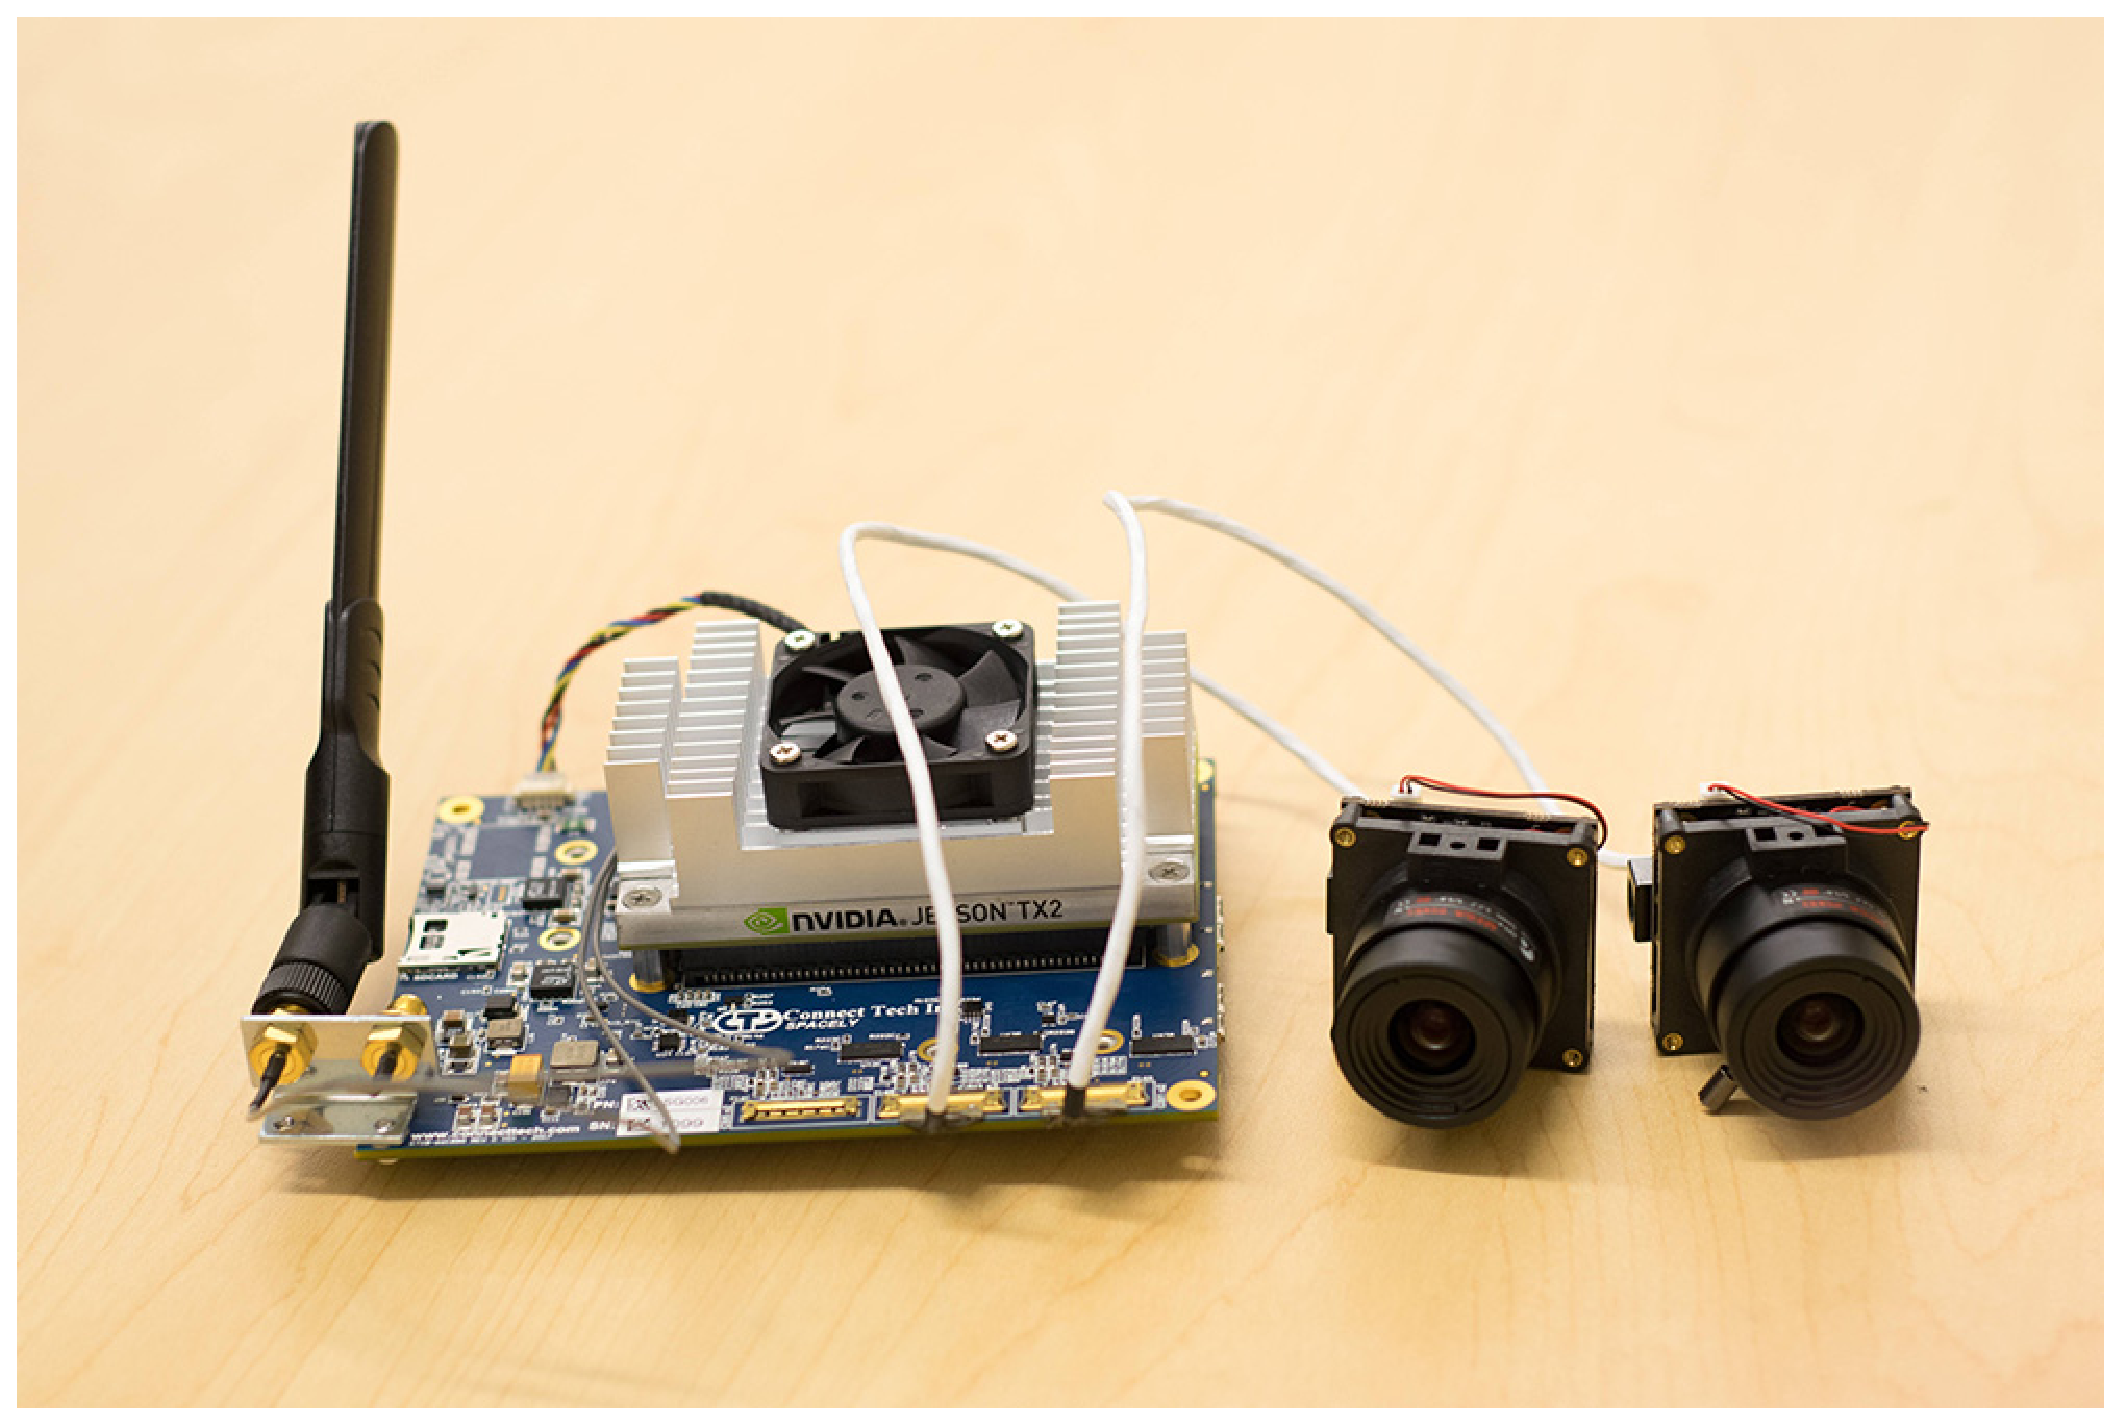
\includegraphics[width=10cm]{images/spacely.eps}
	\caption{TX2 mounted on the Spacely Carrier Board with two Leopard CSI cameras attached. \label{overflow}}
\end{figure}



\nocite{*}
\newpage
\bibliographystyle{ieeetr}
\bibliography{WMPR_Group51}
\end{document}
